% Methods

\textframe{How do I Machine Learning?}

\begin{slide}{Methods}
  \centering
  \Large
  \pause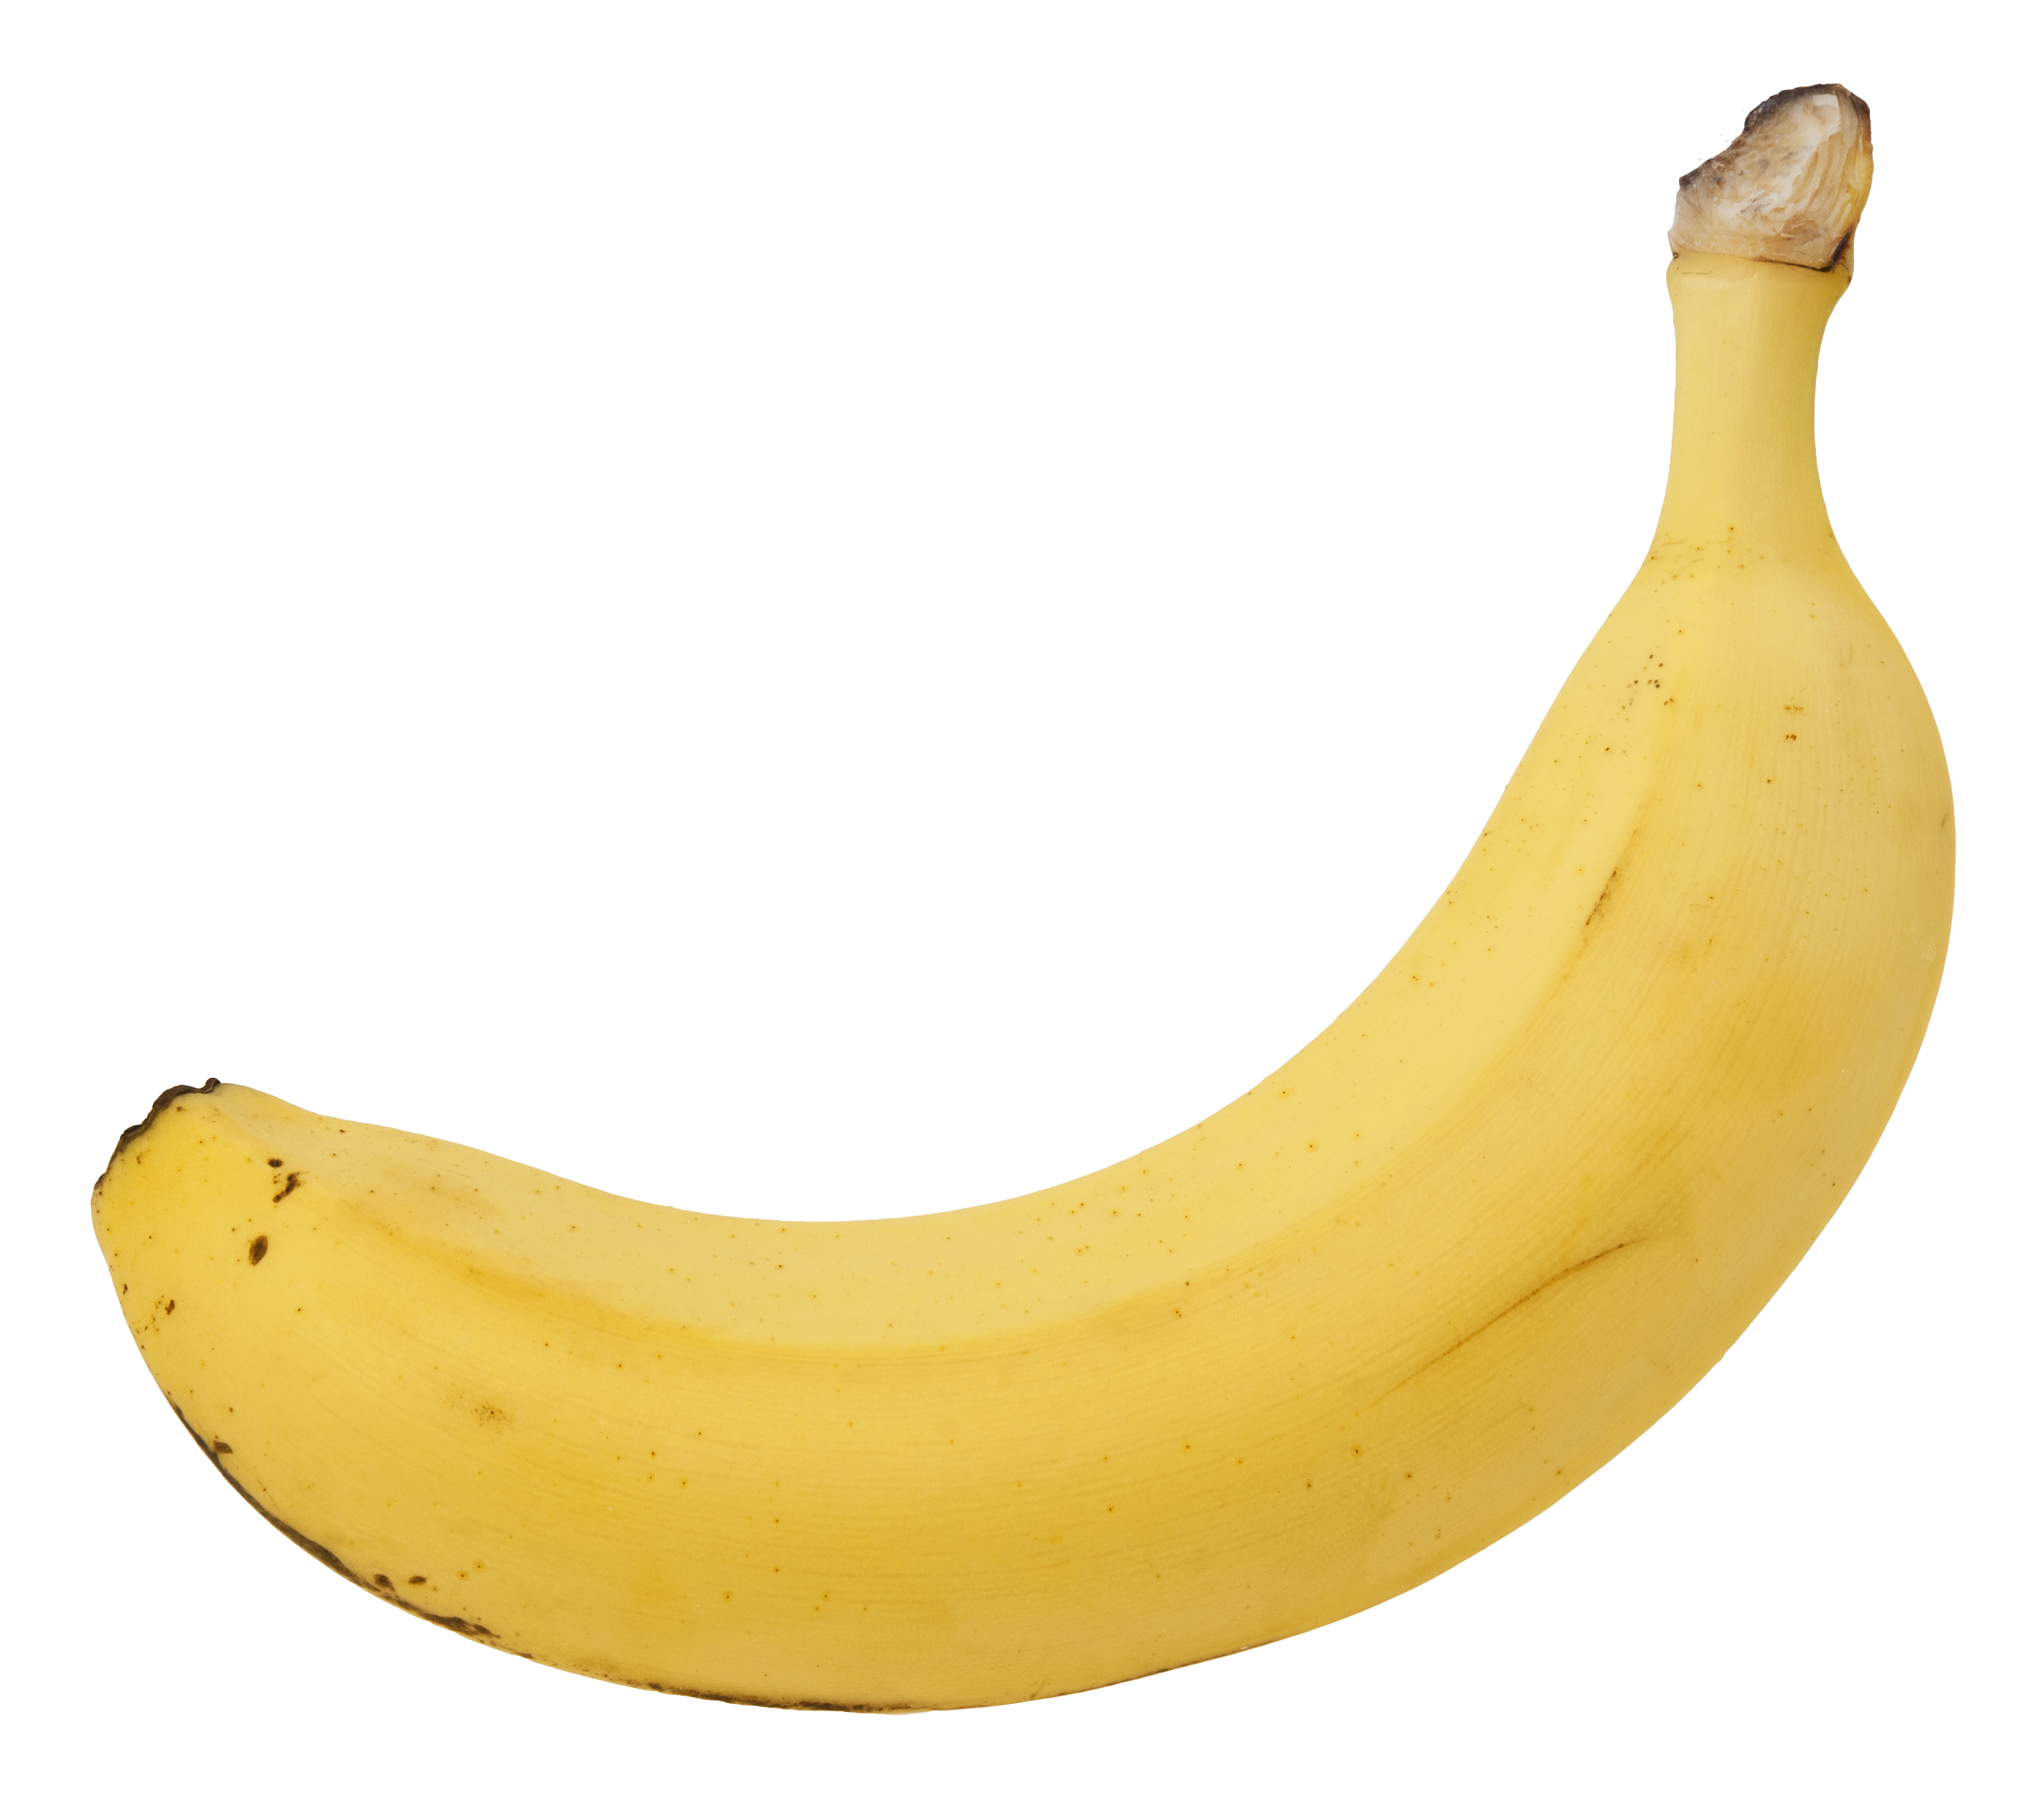
\includegraphics[scale=0.05, trim={0, 0, 0, 4cm}, clip]{banana}\\
  \vspace{0.4cm}
  \pause$\mathbf{b} = (R, G, B)^\top$\\
  \vspace{0.3cm}
  \pause$f: \mathbf{b} \mapsto \text{market price} \in \mathbb{R}$
\end{slide}

\begin{slide}{Methods: Features}
\begin{columns}
  \begin{column}{0.5\textwidth}
  \begin{itemize}
    \item<2-> The components of each vector $\mathbf{b}$ are our \textbf{features}
    \item<3-> Each feature represents one axis in space
    \vspace{2.4cm}
  \end{itemize}
  \end{column}
  \begin{column}{0.5\textwidth}
    \begin{tikzpicture}
      \onslide<4-6>{
      % R Axis
      \draw [->]
            (0, 0, 0) node [left] {$0$}
         -- (2.5, 0, 0) node [right] {$255$}
            node [pos=0.85, above, color=Red] {$R$};
      } \onslide <5-6> {
      % G Axis
      \draw [->]
            (0, 0, 0)
         -- (0, 4, 0) node [above] {$255$}
            node [pos=0.9, left, color=Green] {$G$};
      } \onslide <6> {
      % B Axis
      \draw [->]
            (0, 0, 0)
         -- (0, 0, 4) node [below left] {$255$}
            node [pos=0.9, above, color=ProcessBlue] {$B$};
      }
      % Grid
      % \draw [step=0.5, help lines] (0, 0, 0) grid (2.5, 4, 0);
      % \begin{scope}[canvas is zy plane at x=0]
      %   \draw [step=0.5, help lines] (0, 0) grid (4, 4);
      % \end{scope}
      % \begin{scope}[canvas is zx plane at y=0]
      %   \draw [step=0.5, help lines] (0, 0) grid (4, 2.5);
      % \end{scope}
    \end{tikzpicture}
  \end{column}
\end{columns}
\end{slide}

\begin{slide}{Methods: Features}
\begin{columns}
  \begin{column}{0.5\textwidth}
  \begin{itemize}
    \item The components of each vector $\mathbf{b}$ are our \textbf{features}
    \item Each feature represents one axis in space
    \item<3-> Each feature should contribute to some extent to the output value (market price)
  \end{itemize}
  \end{column}
  \begin{column}{0.5\textwidth}
    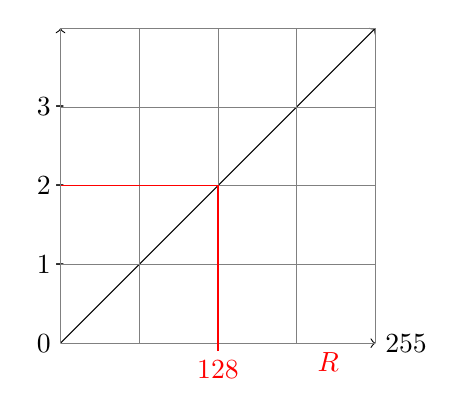
\begin{tikzpicture}
      % R Axis
      \draw [->]
            (0, 0) node [left] {$0$}
         -- (4, 0) node [right] {$255$}
            node [pos=0.85, below, color=Red] {$R$};

      % price axis
      \draw [->]
            (0, 0)
         -- (0, 4)
            node [pos=0.9, left, color=Goldenrod] {$\bitcoin$};

      % Ticks
      \foreach \i in {1, ..., 3} {
        \draw (0, \i) node {-} node [left] {\i};
      }

      % Function
      \draw [domain=0:4, ->] plot(\x, \x);

      % Grid
      \draw [help lines] (0, 0) grid (4, 4);

      \only<2->{
      % Price line
      \draw [color=Red] (2, -0.1) node [below] {128}
         -- (2, 2)
         -- (0, 2);
         }
    \end{tikzpicture}
  \end{column}
\end{columns}
\end{slide}

\begin{slide}{Methods: Features}
  \begin{columns}
  \begin{column}{0.55\textwidth}
  \begin{itemize}
    \item<1-> To model this, we apply a weight $w_i$ to each component $b_i$
    \item<2-> Positive values of $w_i$ \emph{encourage} positive values of $b_i$
    \item<3-> Negative values of $w_i$ \emph{inhibit} $b_i$
    \item<4-> We add a bias $c$ as an offset % e.g. negative bias means we expect a minimum amount for the sum of each component
    \item<5-> We expect our algorithm to learn $\mathbf{w}$ and $c$% We initialize them to zero, or more commonly, random values (e.g. from a uniform or gaussian distribution)
  \end{itemize}
  \end{column}
  \begin{column}{0.45\textwidth}
    \centering
    \only<1-3> {$f(\mathbf{b}) = w_1b_1 + w_2b_2 + w_3b_3$}
    \only<4> {$f(\mathbf{b}) = w_1b_1 + w_2b_2 + w_3b_3 + c$}
    \only<5> {$f(\mathbf{b}) = \mathbf{w}^\top\mathbf{b} + c$}
  \end{column}
\end{columns}
\end{slide}

% Training, Validation, Test set
% You're studying for an exam and do practice problems until you get good results
% Then you try out last year's exam, which is supposed to be a test of how well you studying generalized to new problems
% You fail half the questions, so you go back and memorize all the answer for those specific examples that you failed at in the exam from last year
% Now you have good accuracy for your practice examples, and good accuracy for this specific exam from last year, but this still doesn't mean that you're well prepared for this year's exam and entirely new problems. You won't generalize well.
% Because you leaked in the specifics of last year's exam into your studying, rather than trying to develop the methods necessary to tackle any kinds of problems.
% First thing: design matrix
% Second thing: test, validation, training set
\begin{frame}[fragile]{Methods: Data}
  \begin{itemize}
    \item To make our algorithm learn, we need to feed it (lots of) data
    \item<2-> In practice, we organize our data into a matrix $\mathbf{D} \in
    \mathbb{R}^{n \times k}$
  \end{itemize}
  \only<-2>{\vspace{3.7cm}}
  \only<3> {
    \begin{center}
    \begin{blockarray}{cccc}
      & R & G & B \\
      \begin{block}{c[ccc]}
        & 34 & 147 & 73\\
        n & 247 & 69 & 13\\
        & 66 & 66 & 66\\
      \end{block}
    \end{blockarray}\\
    \hspace{0.75cm}\textbf{Design Matrix}
  \end{center}
  } \begin{onlyenv}<4>
  \vspace{1cm}
  \begin{lstlisting}
    D = np.array([[34, 147, 37], [247, 69, 13], [66, 66, 66]])
    w = np.random.rand(3, 1)
    b = np.random.randn()
    y = D.dot(w) + b
  \end{lstlisting}
  \vspace{0.7cm}
\end{onlyenv}
\end{frame}

\begin{slide}{Methods: Data}
  \centering
  \begin{tikzpicture}
    \path (3, 4) coordinate [cloud, draw,cloud puffs=10,cloud puff arc=120, aspect=2, inner ysep=1em] (d) node {Data};
    \onslide<2->{
      \path (0, 0) coordinate [
        draw,
        rectangle,
        text centered,
        rounded corners,
        minimum width=2cm,
        minimum height=1.5cm
        ] (tr)
            node [above] {Test Set}
            node [below] {\,\,$60\%$};
      \draw (tr) -- (d);
    }

    \onslide<3->{
    \path (3, 0) coordinate [
        draw,
        rectangle,
        text centered,
        rounded corners,
        minimum width=2.5cm,
        minimum height=1.5cm
        ] (va)
          node [above] {Validation Set}
          node [below] {\,\,$20\%$};
    \draw (va) -- (d);
    }

    \onslide<4->{
    \path (6, 0) coordinate [
        draw,
        rectangle,
        text centered,
        rounded corners,
        minimum width=2.2cm,
        minimum height=1.5cm
        ] (te)
          node [above] {Training Set}
          node [below] {\,\,$20\%$};
    \draw (te) -- (d);
    }
  \end{tikzpicture}
\end{slide}

\begin{slide}{Methods: Measuring Performance}
\begin{itemize}
  \pitem Need a way to evaluate the performance of our algorithm ($P$)
  \pitem Once we know how well it is performing, we can update it
  \pitem The loss function we use depends on the learning task
\end{itemize}
\pause
\vspace{0.5cm}
$$L(\mathbf{y}, \mathbf{\hat{y}}) \in \mathbb{R}$$
\end{slide}

\begin{slide}{Methods: Measuring Performance}
  \centering
  {\Large Regression}

  \onslide<2->{
  $$
  \begin{sbmatrix}{\mathbf{D}}
    34 & 147 & 73\\
    247 & 69 & 13\\
    66 & 66 & 66\\
  \end{sbmatrix}
  \times
  \begin{sbmatrix}{\mathbf{w}}
    w_1 \\
    w_2 \\
    w_3
  \end{sbmatrix} +\, c =
  \begin{sbmatrix}{\mathbf{y}}
    y_1 \\
    y_2 \\
    y_3
  \end{sbmatrix}
  \xrightarrow{Target}
  \begin{sbmatrix}{\mathbf{\hat{y}}}
    \hat{y_1} \\
    \hat{y_2} \\
    \hat{y_3}
  \end{sbmatrix}
  $$
  }
  \onslide<3>{
  % Let k be the number of features
  $$
  L(\mathbf{y}, \mathbf{\hat{y}}) = MSE(\mathbf{y}, \mathbf{\hat{y}}) = \frac{1}{k}\sum_{i=1}^k(y_i - \hat{y_i})^2
  $$
  }
\end{slide}

\begin{slide}{Methods: Measuring Performance}
  \centering
  {\Large Regression}
  \vspace{0.5cm}

  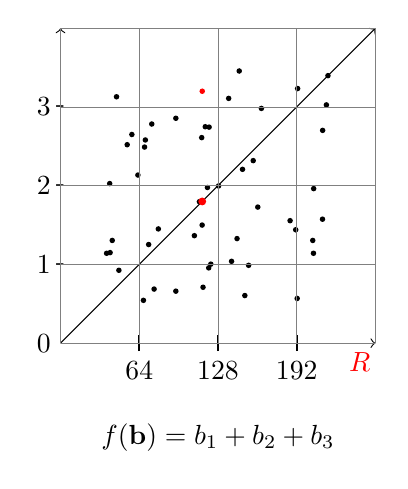
\begin{tikzpicture}
    % R Axis
    \draw [->]
          (0, 0) node [left] {$0$}
       -- (4, 0)
          node [pos=0.95, below, color=Red] {$R$};

    % price axis
    \draw [->]
          (0, 0)
       -- (0, 4)
          node [pos=0.9, left, color=Goldenrod] {$\bitcoin$};

    % Ticks
    \foreach \i/\j in {1/64, 2/128, 3/192} {
      \draw (0, \i) node {-} node [left] {\i};
      \draw [thick] (\i, -0.1) node [below] {\j} -- (\i, 0.1);
    }

    % Data
    \onslide<2->{
    \foreach \i in {1, ..., 50} {
      \fill [black, thin] ({2+rand*1.5}, {2+rand*1.5}) circle [radius=1pt];
    }
    }

    \onslide<3->{
    % Function
    \draw [domain=0:4, ->] plot(\x, \x);

    % Equation
    \draw (2, -1.2) node {$f(\mathbf{b}) = b_1 + b_2 + b_3$};
    }

    \onslide<4->{
      \fill [color=red] (1.8, 1.8) circle [radius=0.05cm];
    }

    \onslide<5->{
      \fill [red] (1.8, 3.2) circle [radius=1pt];
    }

    % Grid
    \draw [help lines] (0, 0) grid (4, 4);
  \end{tikzpicture}
\end{slide}

% \begin{slide}{Methods: Measuring Performance}
%   \centering
%   {\Large Binary Classification}
%   \vspace{0.5cm}
%
%   \begin{itemize}
%     \item<1-> We can transform any regression task into a binary classification task
%     \item<2-> Simply set a threshold
%     \item<3-> Need to squash our $y$ into the range $[0, 1]$
%   \end{itemize}
%   \only<-3>{\vspace{1.65cm}}
%   \only<-4>{\vspace{0.4cm}}
%   \only<4>{
%   $$\sigma(z) = \frac{1}{1 + e^{-z}}$$
%   \vspace{0cm}\\
%   \emph{Sigmoid (Logistic)} Function
%   }
%
%   \only<5>{
%   \begin{figure}
%     \begin{tikzpicture}[scale=0.55]
%     \begin{axis}[
%       legend style={empty legend, draw=none, anchor=north},
%       axis lines=center,
%       xmin=-7, xmax=7,
%       ymin=0, ymax=1.3,
%       ytick={0.5, 1}
%       % grid
%     ]
%
%       \addplot[domain=-7:7, samples=100]{1/(1 + exp(-x))};
%
%       \addlegendentry{$\sigma(z)$}
%     \end{axis}
%     \end{tikzpicture}
%   \end{figure}
%   }
% \end{slide}
%
% \begin{slide}{Methods: Measuring Performance}
%   \centering
%   {\Large Binary Classification}
%   \vspace{0.5cm}
%
%   $$\begin{sbmatrix}{\mathbf{y}}3.141 \\ -2.718 \\ 0.707\end{sbmatrix}
%   \pause
%   \xrightarrow{\sigma}
%   \begin{sbmatrix}{\sigma(\mathbf{y})}0.957 \\  0.062 \\  0.670\end{sbmatrix}
%   \pause
%   \xrightarrow{> 0.5}
%   \begin{sbmatrix}{\mathbf{y}_b}1 \\ 0 \\  1\end{sbmatrix}
%   \pause
%   \xrightarrow{Target}
%   \begin{sbmatrix}{\mathbf{\hat{y}}}
%     \hat{y_1} \\
%     \hat{y_2} \\
%     \hat{y_3}
%   \end{sbmatrix}
%   $$
%
%   % # of times the 1 was correct + # times the 0 was correct / all examples
%   \pause
%   $L(\mathbf{y}_b, \mathbf{\hat{y}}) = ACC(\mathbf{y}_b, \mathbf{\hat{y}}) = \frac{TP + TN}{n}$
% \end{slide}
%
% \begin{frame}[fragile]{Methods: Measuring Performance}
%   \centering
%   {\Large Binary Classification}
%   \vspace{0.5cm}
%   \begin{lstlisting}
%     y = np.array([3.141, -2.718, 0.707])
%     sigmoid = lambda z: 1 / (1 + np.exp(-z))
%     sigmoid = np.vectorize(sigmoid)
%     y_s = logistic(y)
%     y_b = y_s > 0.5 # [True, False, True]
%     acc = np.mean(y_b == y_hat)
%   \end{lstlisting}
% \end{frame}
%
% \begin{slide}{Methods: Measuring Performance}
%   \centering
%   {\Large Multi-Class Classification}
%   \vspace{0.5cm}
%   \begin{itemize}
%     \pitem More than two possible classes
%     \pitem $\mathbf{y}$ becomes a matrix $\mathbf{Y}$ % Imagine we just had three separte linear regression classifiers
%     \pitem $\mathbf{\hat{y}}$ becomes a matrix $\mathbf{\hat{Y}}$
%     \pitem Each row $\mathbf{\hat{Y}}_i$ is \emph{one-hot encoded}: $(0, \dots, 1, \dots, 0)^\top$
%   \end{itemize}
% \end{slide}
%
% \begin{slide}{Methods: Measuring Performance}
%   \centering
%   {\Large Multi-Class Classification}
%   \vspace{0.5cm}
%   $$
%   \begin{blockarray}{cccc}
%     & \text{Cat} & \text{Banana} & \text{Spaceship} \\
%     \begin{block}{c[ccc]}
%     & 0.493 & 7.791 & 8.649 \\
%     n & 1.232 & 6.900 & 9.881 \\
%     & 0.087 & 1.996 & 2.062 \\
%     \end{block}
%     & & \mathbf{Y}& &
%   \end{blockarray}
%   \xrightarrow{\text{Target}}
%   \begin{sbmatrix}{\mathbf{\hat{Y}}}
%     0.0 & 0.0 & 1.0 \\
%     1.0 & 0.0 & 0.0 \\
%     0.0 & 1.0 & 0.0
%   \end{sbmatrix}
%   $$
%
%   \begin{itemize}
%     \pitem $\mathbf{\hat{Y}}$ can be interpreted as the likelyhood of each class
%     \pitem $\mathbf{Y}$ can be interpreted as random numbers
%     \pitem We want to turn $\mathbf{Y}$ into a probability distribution
%   \end{itemize}
% \end{slide}
%
% \begin{slide}{Methods: Measuring Performance}
%   \centering
%   {\Large Multi-Class Classification}
%   \vspace{0.5cm}
%   $$\softmax(\mathbf{Y}_i)_j = \frac{\exp\{\mathbf{Y}_{i,j}\}}{\sum_j \exp\{\mathbf{Y}_{i,j}\}}$$
%   \pause
%   fancy version of
%   \pause
%   $$\text{normalize}(\mathbf{Y_i})_j = \frac{\mathbf{Y}_{i,j}}{\sum_j \mathbf{Y}_{i,j}}$$
%   \pause
%   % Each value is smaller than the sum
%   % The sum of the parts give 1
%   e.g. for $\mathbf{y} = (1, 2, 3)^\top$
%   $$\text{normalize}(\mathbf{y})_2 = \frac{2}{1 + 2 + 3} \approx 0.333$$
% \end{slide}
%
% \begin{slide}{Methods: Measuring Performance}
%   \centering
%   \frameheader{Multi-Class Classification}
%   $$\mathbf{Y}_s = \softmax(\mathbf{Y}) =
%     \begin{bmatrix}
%       0.0002 & 0.2977 & 0.7021 \\
%       0.0002 & 0.0483 & 0.9515 \\
%       0.0669 & 0.4512 & 0.482
%     \end{bmatrix}
%   $$
%   \pause
%   Now we can ask: How similar is $\mathbf{Y}_s$ to $\mathbf{\hat{Y}}$?
% \end{slide}
%
% \begin{slide}{Methods: Measuring Performance}
%   \centering
%   \frameheader{Multi-Class Classification}
%   \vspace{0.5cm}
%
%   The \textbf{Cross Entropy} $H(\mathbf{Y}_s, \mathbf{\hat{Y}})$ gives us the answer:
%   $$H(\mathbf{Y}_{s_i}, \mathbf{\hat{Y}}_i) = -\sum_{j=1}^n \mathbf{\hat{Y}}_{i,j} \log(\mathbf{Y}_{s_{i,j}})$$
%   Finally, our loss is the mean over all examples:
%   $$L(\mathbf{Y}_s, \mathbf{\hat{Y}}) = \frac{1}{n}\sum_{i=1}^n H(\mathbf{Y}_{s_i}, \mathbf{\hat{Y}}_i)$$
% \end{slide}

\begin{slide}{Methods: Weight Update}
  \centering
\begin{itemize}
  \pitem Through $L(\mathbf{y}, \mathbf{\hat{y}})$ we know how our algorithm is performing
  \pitem We can compute its rate of change (derivative)
  \pitem Move our weights in the opposite direction
  \pitem Next time, the loss will be smaller
  \pitem We repeat this, until we're happy
\end{itemize}

\pause
\vspace{1cm}
\textbf{This is the core idea behind Machine Learning}
\end{slide}

\begin{slide}{Methods: Weight Update}
  \centering
  \begin{itemize}
    % L is the per-example loss
    \pitem $L(\mathbf{y}, \mathbf{\hat{y}})$ depends on $\mathbf{y}$ and $\mathbf{\hat{y}}$, but \emph{also} $\mathbf{w}$: $L(\mathbf{y}, \mathbf{\hat{y}}; \mathbf{w})$
    \pitem We are interested in the way the loss changes w.r.t to the \emph{weights} $\mathbf{w}$ (and bias $b$) % but we can just think of b as an extra entry in the vector w if we adjust our design matrix accordingly
    \pitem Moreover, we think in terms of entire batches, not single examples
    \pitem We need new notation:
  \end{itemize}
  \vspace{0.5cm}
  \pause
  We can think of $\mathbf{Y}, \mathbf{\hat{Y}}$ as being \emph{constant} and write:
  % Remember that Y contains the results of our prediction, which we defined as the product of weights and our input features x. So we just keep the weights constant. This is exactly what the partial derivative does. In a sense, L is actually dependent of x *and* w, so when we compute the partial derivative of L w.r.t to w, we're keeping x constant. We just make this explicit here.
  $$J(w) = \frac{1}{n}\sum_{i=1}^n L(\mathbf{Y}_i, \mathbf{\hat{Y}}_i; w)$$
  % This is really just a notational aid. When we compute the derivative, we're still actually computing partial derviatives, not total derivatives
  % The mean here is actually the expetance in the loss
\end{slide}

% Hier erstmal alles erklaeren (weight update)
\begin{slide}{Methods: Weight Update}
  \centering
  % Note that w is actually a multidimensional vector, so this plot is not quite precise, unless we assume that w consists of only one component
  % Usually you will see three-dimensional plots
  \begin{tikzpicture}[scale=0.8]
    % weight axis
    \draw [->] (-2.5, 0)
            -- (5, 0) node [below left] {$\mathbf{w}$};

    % loss axis
    \draw [->] (0, -0.5) node [left]{$0$}
            -- (0, 5) node [left] {$J(\mathbf{w})$};

    % No ticks, because we have no units

    % Loss function
    \draw [domain=-2.4:3.15, samples=200] plot (\x, {-0.05*\x^7 + 0.15*\x^6 + 0.25*\x^5 - 0.7*\x^4 - 0.35*\x^3 + 0.5*\x^2 + 0.55*\x + 1.55});

    % Grid
    % \draw [help lines] (-2.5, -0.5) grid (5, 5);

    % Current weights
    \only<2-> {
      \draw [fill=red, thin] (2.3, 2.9) circle [radius=1.5pt];
      \draw [red, dashed] (2.3, -0.1) -- (2.3, 2.85);
    }

    % Tangent
    \only<3-> {
      \draw [dotted] (1.8, 0.5) -- ++(78.5:4.75);
    }
  \end{tikzpicture}
  \onslide<4-> {
    $$\mathbf{w} \leftarrow \mathbf{w} - \text{rate of change at } \mathbf{w}$$
  }
\end{slide}

% we can think of a uni-variate function as a string, that we can fold up and down like a function f(x)
% for a multi-variate function, like a two-variate function f(x, y), we can think of the function not as a string, but as a carpet. We can manipulate the carpet's two-dimensional shape in both of its two dimension. Fo example, we can make a hump in the carpet (hill, like __/-\__), then we are changing it in the one (x) dimension. We can observe a change of the function in this dimension. However, in this hump it is not changing in the other y dimension. But, we can additioanlly pull the hump up on the other side of the carpet (behind the __/-\__). Then we are changing it in the other, second dimension which we can observere, calculate and study. But when we are only concerned with the change of the function in the one dimension, in the way the hump is changing the function up and down in dependence of the x component, then we do not care about how the y dimension is pulling the carpet/hump up in the y dimension. So with a partial derivative we get a view of how the carpet is changing only in one of the dimensions. This is done by simply regarding the change in the other dimmension(s) s constant, since a constant will only move the hump up and down but not alter the way the hump changes the functions' value  in the x dimension. The important thing is that constants are lost when taking derivatives, so we are left only with the change of the carpet in onde dimension.

\begin{slide}{Digression: Calculus Recap}
  \begin{itemize}
    \pitem Let's talk about $f$
    \pitem When $f$ depends on one variable $x$, $$f'(x) = \frac{\mathrm{d}f}{\mathrm{d}x}$$ is the \emph{derivative} of $f$ w.r.t. $x$
    \pitem It tells us how $f$ is changing in dependence of $x$
  \end{itemize}
\end{slide}

\begin{slide}{Digression: Calculus Recap}
  \begin{itemize}
    \pitem In $f(x, y) = x + y$ both $x$ and $y$ are influencing $f$'s output
    \pitem We want to know \emph{how} they are influencing $f$ independently
    % We want to know, for a given x, by what amount is f cu
    \pitem The partial derivative $\frac{\partial f}{\partial x}$ gives us a \emph{view} of $f$
    \pitem In this view, all variables but $x$ are constant % And thus do not influence f's rate of change
    \pitem Thus, we can extract the change of $f$ w.r.t. to $f$
  \end{itemize}
\end{slide}

\begin{slide}{Digression: Calculus Recap}
  \begin{itemize}
    \pitem Let $f: \mathbb{R}^n \rightarrow \mathbb{R}$ be a scalar-valued function \emph{taking} a vector $\mathbf{x}$ as input.
    \pitem Then $$\frac{\partial f}{\partial v_i}$$ is a partial derivative, and
    \pitem $\nabla f$ the vector containing the partial derivatives of $w$: $$\nabla f = \left(\frac{\partial f}{\partial v_1}, \dots, \frac{\partial f}{\partial v_n}\right)^\top$$
    \pitem $\nabla f$ is called the \emph{gradient} of $f$
  \end{itemize}
\end{slide}

\begin{slide}{Methods: Weight Update}
  \centering
  % Note that w is actually a multidimensional vector, so this plot is not quite precise, unless we assume that w consists of only one component
  % Usually you will see three-dimensional plots
  \begin{tikzpicture}[scale=0.8]
    % weight axis
    \draw [->] (-2.5, 0)
            -- (5, 0) node [below left] {$\mathbf{w}$};

    % loss axis
    \draw [->] (0, -0.5) node [left]{$0$}
            -- (0, 5) node [left] {$J(\mathbf{w})$};

    % No ticks, because we have no units

    % Loss function
    \draw [domain=-2.4:3.15, samples=200] plot (\x, {-0.05*\x^7 + 0.15*\x^6 + 0.25*\x^5 - 0.7*\x^4 - 0.35*\x^3 + 0.5*\x^2 + 0.55*\x + 1.55});

    % Grid
    % \draw [help lines] (-2.5, -0.5) grid (5, 5);

    % Current weights
    \draw [fill=red, thin] (2.3, 2.9) circle [radius=1.5pt];
    \draw [red, dashed] (2.3, -0.1) -- (2.3, 2.85);

    \draw [dotted] (1.8, 0.5) -- ++(78.5:4.75);
  \end{tikzpicture}
  % First explain what we are trying to do
  \onslide<2>{
  $$\nabla J(w) = \frac{1}{n}\sum_{i=1}^n \nabla_w L(\mathbf{Y}, \mathbf{\hat{Y}}_i; w)$$
  }
  %
  % Remember that we hold Y and Y_hat constant,
\end{slide}

\begin{slide}{Methods: Weight Update}
  \centering
  \begin{itemize}
    \item<1-> This method of updating weights is called \emph{Gradient Descent} (GD)
    \item<2-> It adds a \emph{hyperparameter} $\alpha$ as a knob to tweak: $$w \leftarrow w - \alpha \nabla J(w)$$
    \item<3-> $\alpha$ is called the \emph{learning rate}
    \item<4-> Often, we will apply a decay to it
  \end{itemize}
\end{slide}

\begin{slide}{Methods: Weight Update}
  \centering
  \begin{itemize}
    \item<1-> The goal of GD is to find the weights that minimize the loss for our training data
    \item<2-> The theoretical goal is to find the global minimum of $J(w)$
    \item<3-> In practice, we most often use \emph{Stochastic Gradient Descent}
    % The idea is: GD is just an estimate of where the weights should go. The weight update is not actually a mathematically exact operation. If you think about, we're subtracting the speed from the distance (since derivative of distance/time is speed). What does that even mean? Physicists won't even talk to you even more when you tell them that you're subtracting two values with different unit. So since GD is just an estimate, we can also make that estimate with a sample of our data and it will be stochastically valid.
    \item<4-> Many variations and alternatives exist
  \end{itemize}
  \vspace{0.3cm}
  \onslide<5->{
  $$\nu = \gamma\nu + \alpha\nabla J(w)$$
  $$w \leftarrow w - \nu$$
  \textbf{Momentum Optimizer}
  % The momentum optimizer takes previous gradients into account, or the current "trend of the gradient". This can be especially helpful to overcome local optima. Think of the gradient as a ball rolling down a hill, when the slope is steep, adding the previous gradient will make the weight update go back further, as if the ball had caught on momentum from rolling down the hill. This way, when there is a slight hill upwards after the local minimum, the ball will have gathered enough momentum to overcome the hill (i.e. the weight update will move w past the hill). Because then \gamma\nu will be, say, very negative and the new gradient very (-\nabla J) slightly positive, in total, the negative will prevail and our ball will roll past the local optimum.
  }

\end{slide}

\begin{slide}{Methods: Regularization}
  \begin{itemize}
    \pitem We want our models to \emph{generalize}
    \pitem Parameters should not specialize too much to training data
    \pitem \emph{Regularization} is the art of finding a tradeoff between
    \begin{itemize}
      \pitem training error
      \item generalization error
    \end{itemize}
    \pitem We try to influence a model's \emph{capacity}
  \end{itemize}
\end{slide}

% Idea: the dots are our training data
% Our whole data set lies somewhere around the quadratic
\begin{slide}{Concepts: Model Capacity}
  \centering
  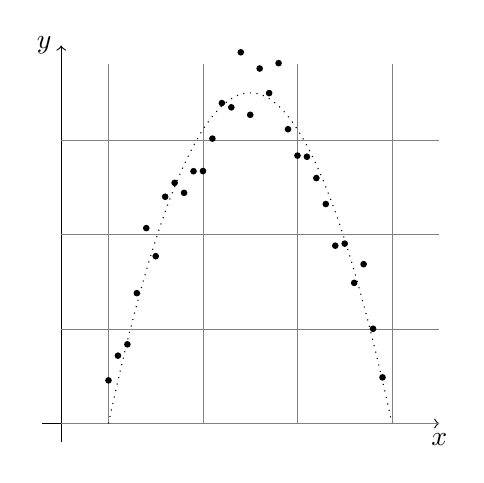
\begin{tikzpicture}[
      scale=1.2,
      declare function={f(\x) = -14/9*\x^2 + 42/9*\x;}
    ]
    % x axis
    \draw [->] (-0.7, 0) -- (3.5, 0) node [below] {$x$};

    % y axis
    \draw [->] (-0.5, -0.2) -- (-0.5, 4) node [left] {$y$};

    % grid
    \draw [help lines] (-0.5, 0) grid (3.5, 3.8);

    % Function
    \draw [domain=0:3, samples=100, dotted] plot (\x, {f(\x)});

    % Some training points
    \foreach \x in {0, 0.1, ..., 3} {
      \fill [black] (\x, {f(\x) + rand*0.5 + 0.05}) circle [radius=1pt];
    }
  \end{tikzpicture}

  \vspace{0.3cm}
\end{slide}

\begin{slide}{Concepts: Model Capacity}
  \centering
  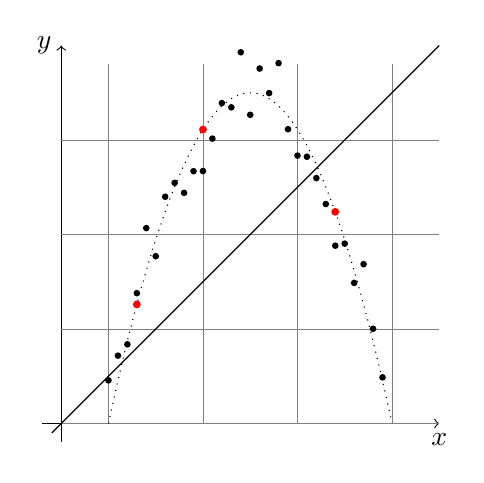
\begin{tikzpicture}[
      scale=1.2,
      declare function={f(\x) = -14/9*\x^2 + 42/9*\x;}
    ]
    % x axis
    \draw [->] (-0.7, 0) -- (3.5, 0) node [below] {$x$};

    % y axis
    \draw [->] (-0.5, -0.2) -- (-0.5, 4) node [left] {$y$};

    % grid
    \draw [help lines] (-0.5, 0) grid (3.5, 3.8);

    % Function
    \draw [domain=0:3, samples=100, dotted] plot (\x, {f(\x)});

    % Some test points
    \path [red] (1, {f(1)}) coordinate [fill, circle, inner sep=1pt] (a);
    \path [red] (0.3, {f(0.3)}) coordinate [fill, circle, inner sep=1pt] (b);
    \path [red] (2.4, {f(2.4)}) coordinate [fill, circle, inner sep=1pt] (c);

    % Some training points
    \foreach \x in {0, 0.1, ..., 3} {
      \fill [black] (\x, {f(\x) + rand*0.5 + 0.05}) circle [radius=1pt];
    }

    \only<2->{
      \draw [domain=-0.6:3.5] plot (\x, {\x+0.5});
    }
  \end{tikzpicture}

  \onslide<2->{
    Underfitting (low capacity)
    % Will have very bad training error
    % And also a very bad generalization error
    % Theoretically, it should generalize very well
    % But only if we assume we want to match all possible data
    % If we know our data will be approximately quadratic
    % Then we should make use of that knowledge
    % Else the generalization error will be bad too
  }
\end{slide}

\begin{slide}{Concepts: Model Capacity}
  \centering
  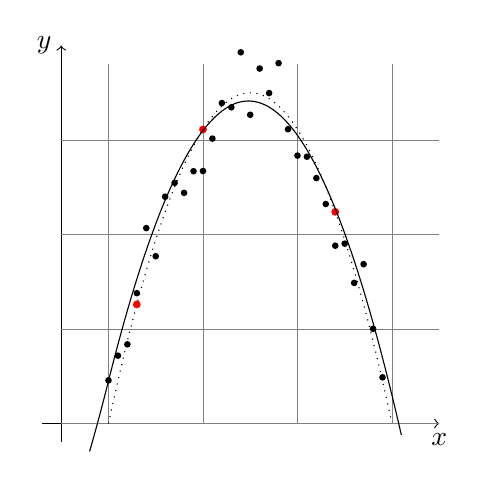
\begin{tikzpicture}[
      scale=1.2,
      declare function={f(\x) = -14/9*\x^2 + 42/9*\x;}
    ]
    % x axis
    \draw [->] (-0.7, 0) -- (3.5, 0) node [below] {$x$};

    % y axis
    \draw [->] (-0.5, -0.2) -- (-0.5, 4) node [left] {$y$};

    % grid
    \draw [help lines] (-0.5, 0) grid (3.5, 3.8);

    % Function
    \draw [domain=0:3, samples=100, dotted] plot (\x, {f(\x)});

    % Some test points
    \path [red] (1, {f(1)}) coordinate [fill, circle, inner sep=1pt] (a);
    \path [red] (0.3, {f(0.3)}) coordinate [fill, circle, inner sep=1pt] (b);
    \path [red] (2.4, {f(2.4)}) coordinate [fill, circle, inner sep=1pt] (c);

    % Some training points
    \foreach \x in {0, 0.1, ..., 3} {
      \fill [black] (\x, {f(\x) + rand*0.5 + 0.05}) circle [radius=1pt];
    }

    \draw [domain=-0.2:3.1, samples=100] plot (\x, {-1.35*\x^2 + 4*\x + 0.45});
  \end{tikzpicture}

  Just Right (optimal capacity)
\end{slide}

\begin{slide}{Concepts: Model Capacity}
  \centering
  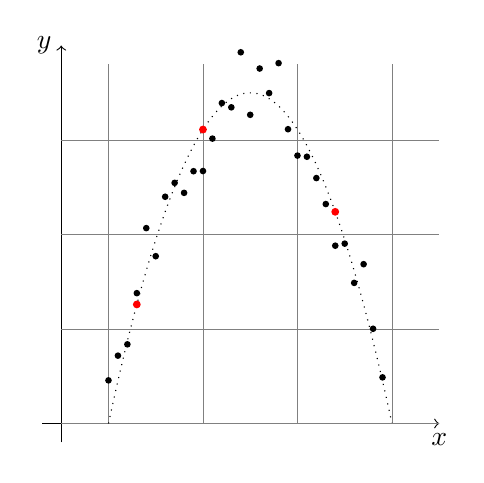
\begin{tikzpicture}[
      scale=1.2,
      declare function={f(\x) = -14/9*\x^2 + 42/9*\x;}
    ]
    % x axis
    \draw [->] (-0.7, 0) -- (3.5, 0) node [below] {$x$};

    % y axis
    \draw [->] (-0.5, -0.2) -- (-0.5, 4) node [left] {$y$};

    % grid
    \draw [help lines] (-0.5, 0) grid (3.5, 3.8);

    % Function
    \draw [domain=0:3, samples=100, dotted] plot (\x, {f(\x)});

    % Some test points
    \path [red] (1, {f(1)}) coordinate [fill, circle, inner sep=1pt] (a);
    \path [red] (0.3, {f(0.3)}) coordinate [fill, circle, inner sep=1pt] (b);
    \path [red] (2.4, {f(2.4)}) coordinate [fill, circle, inner sep=1pt] (c);

    % Some training points
    \foreach \x in {0, 0.1, ..., 3} {
      \fill [black] (\x, {f(\x) + rand*0.5 + 0.05}) circle [radius=1pt];
    }

    % \draw [domain=0:3.5, samples=800, /pgf/fpu,/pgf/fpu/output format=fixed] plot (\x, {-0.6904015551*\x^8 + 10.89843224*\x^7 - 69.51522312*\x^6 + 229.1182621*\x^5 - 413.7646904*\x^4 + 399.5064624*\x^3 - 185.9487975*\x^2 + 33.50595212*\x + 7.169728633*10^-8});
  \end{tikzpicture}

  Overfitting (too high capacity)
\end{slide}

\begin{slide}{Methods: Regularization}
  \begin{align*}
  f(x) &= 0x^8 + 0x^7 + 0x^6\\
       &+ 0x^5 + 0x^4 + 0x^3\\
       &- 1.56x^2  + 4.67x + 0\\
  \vspace{1cm}\\
  g(x) &= -0.69 x^8 + 10.90 x^7 - 69.52 x^6\\
       &+ 229.12 x^5 - 413.77  x^4 + 399.50 x^3\\
       &- 185.95 x^2 + 33.51 x + 7.17 \cdot 10^{-8}
  \end{align*}
  % Large coefficients = large slopes = badass polynomials
\end{slide}

\begin{slide}{Methods: Regularization}
  \begin{itemize}
    \item We can keep our polynomial from getting too funky by keeping weights small
    \pitem We do so by \emph{adding the weights to the cost}

    $$J(w) = MSE(\mathbf{y}, \mathbf{\hat{y}}) + \lambda (\mathbf{w}^\top\mathbf{w})$$\\
    \vspace{0.1cm}
    % We square the weights because we want their magnitude
    \pitem Our algorithm must make a tradeoff between
    \begin{itemize}
      \pitem Minimizing the training error (make weights large)
      \item Keeping the cost small (make weights small)
    \end{itemize}
    \pitem We thus reduce the capacity by \emph{favoring} certain functions over others
  \end{itemize}
\end{slide}
